You are considering implementing the proportional control system shown below. The desired specifications are a settling time of $\ts \leq 2.3$ s and a rise time of $\tr \leq 1$ s. 
\begin{center}
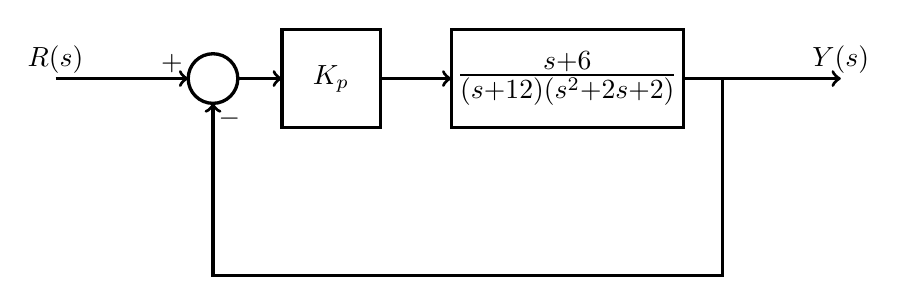
\begin{tikzpicture}[scale=1,inner sep=0pt,outer sep=0pt,very thick,
sysblock/.style={draw,rectangle,inner sep=2pt,minimum width=1.25cm,minimum height=1.25cm,very thick}]
\draw (2,0) node[draw,circle] (sum1) {$\rule{0pt}{18pt}$};
\draw (3.5,0) node[sysblock] (Kp) { $K_{p}$};
\draw (6.5,0) node[sysblock] (G) {\Large $\frac{s+6}{\left(s+12\right)\left(s^2+2s+2\right)}$};
\draw[->] (0,0) node[above=2pt] {$R(s)$} -- (sum1.180) node[above left=2pt] {$+$};
\draw[->] (sum1.0) --  (Kp);
\draw[->] (Kp) -- (G.180);
\draw[->] (G.0) -- ++(2,0) node[above=2pt] {$Y(s)$};
\draw[->] (G.0) ++(0.5,0) -- ++(0,-2.5) -| (sum1.-90) node[below right=2pt] {$-$};
\end{tikzpicture}
\end{center}

\begin{enumerate}[(a)]
%\setlength{\itemsep}{0.5in}
%\setlength{\parskip}{0pt}
%\setlength{\parsep}{0pt}
\item Sketch the root locus on the complex plane.  Please mark and label the Im$\{s\}$ and Re$\{s\}$ axis at important values.
%\begin{center}
%\begin{tikzpicture}[scale=1.0]
%\draw[->] (0,0) -- (10,0) node[above]{Re$\{s\}$};
%\draw[->] (8,-4) -- (8,4) node[right]{Im$\{s\}$};
%\end{tikzpicture}
%\end{center}
\item Sketch the appropriate regions in the complex plane where the dominant closed loop poles should lie for all specifications to be met. Can all
the specification be met?
\end{enumerate}
